\section{Multiplicadores de Lagrange}

El criterio de la segunda derivada localiza los extremos de una función en el interior de su dominio. En muchos problemas, sin embargo, se busca optimizar una función cuando las variables están sujetas a una o varias condiciones. El método de los multiplicadores de Lagrange resuelve esta clase de problemas sin necesidad de despejar las restricciones.

\subsection{Qué es y para qué sirve}

Un problema de optimización con restricciones consiste en hallar los valores extremos de una función objetivo $f(x, y, z)$ sobre el conjunto de puntos que satisfacen una condición $g(x, y, z) = k$. La condición $g = k$ define una curva o superficie de nivel, y el problema equivale a recorrer ese conjunto buscando los puntos donde $f$ es máxima o mínima.

Situaciones de este tipo aparecen con frecuencia: maximizar el volumen de una caja con área superficial fija, minimizar el costo de un material sujeto a un volumen dado, o encontrar el punto de una superficie más cercano al origen. En todos los casos la variable no puede moverse libremente por el espacio, sino solo sobre el conjunto restringido.

La idea geométrica del método es la siguiente. Al recorrer la curva de restricción $g = k$, la función $f$ crece o decrece según se crucen sus curvas de nivel. En un punto extremo, la curva de restricción es tangente a una curva de nivel de $f$. Como el gradiente es perpendicular a las curvas de nivel, en ese punto de tangencia los gradientes $\nabla f$ y $\nabla g$ son paralelos.

\begin{center}
\shorthandoff{>}
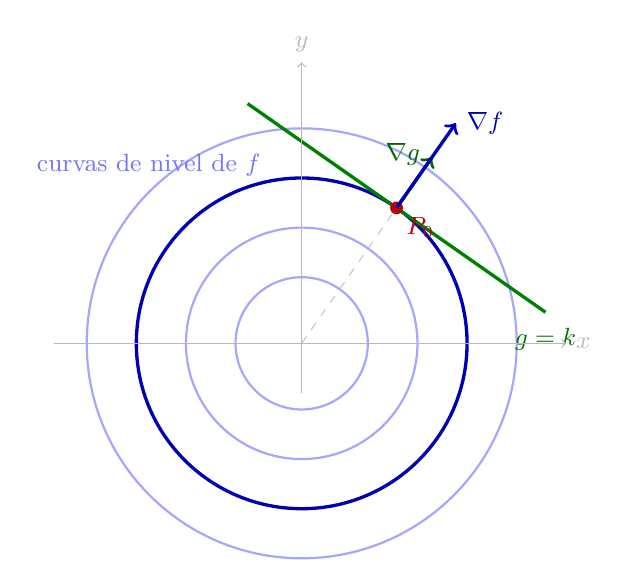
\begin{tikzpicture}[scale=1.05, every node/.style={font=\small}]
    % Curvas de nivel de f (circunferencias concéntricas)
    \draw[blue!35, thick] (0,0) circle (0.8);
    \draw[blue!35, thick] (0,0) circle (1.4);
    \draw[blue!35, thick] (0,0) circle (2.6);
    % Curva de nivel tangente (r=2), resaltada
    \draw[blue!70!black, very thick] (0,0) circle (2.0);
    \node[blue!55] at (-1.85, 2.15) {curvas de nivel de $f$};
    % Punto de tangencia P0 sobre r=2, en el ángulo 55°
    % P0 = (2cos55, 2sin55) = (1.147, 1.638)
    \coordinate (P) at (1.147, 1.638);
    % Restricción g=k: recta tangente a r=2 en P0 (perpendicular al radio)
    % Dirección tangente = (-sin55, cos55) = (-0.8192, 0.5736)
    % Extremos en s = ±2.2:  A=(2.949,0.376), B=(-0.655,2.900)
    \draw[green!50!black, very thick] (2.949, 0.376) -- (-0.655, 2.900);
    \node[green!45!black] at (2.95, 0.05) {$g = k$};
    % Radio punteado hasta P0 (recuerda que el gradiente es radial)
    \draw[gray!45, dashed] (0,0) -- (P);
    % Punto de tangencia
    \fill[red!75!black] (P) circle (2.2pt);
    \node[below right, red!75!black] at (P) {$P_0$};
    % Gradiente de g en P (radial hacia afuera, más corto)
    % dir radial = (cos55, sin55) = (0.5736, 0.8192)
    \draw[->, very thick, green!40!black] (P) -- (1.577, 2.252);
    \node[green!40!black, left] at (1.55, 2.28) {$\nabla g$};
    % Gradiente de f en P (radial hacia afuera, más largo: lambda>1)
    \draw[->, very thick, blue!70!black] (P) -- (1.864, 2.662);
    \node[blue!70!black, right] at (1.88, 2.66) {$\nabla f$};
    % Ejes
    \draw[->, gray!55] (-3,0) -- (3.2,0) node[right] {$x$};
    \draw[->, gray!55] (0,-0.6) -- (0,3.4) node[above] {$y$};
\end{tikzpicture}
\end{center}

En el punto óptimo $P_0$, la restricción es tangente a una curva de nivel de $f$ y los gradientes $\nabla f$ y $\nabla g$ apuntan en la misma dirección (salvo un factor escalar).

\subsection{Método para una restricción}

\begin{mytheorem}{Multiplicadores de Lagrange (una restricción)}
Sean $f$ y $g$ funciones con derivadas parciales continuas. Si $f$ alcanza un extremo local sobre la restricción $g(x, y, z) = k$ en un punto $P_0$ donde $\nabla g(P_0) \neq \mathbf{0}$, entonces existe un escalar $\lambda$, llamado \emph{multiplicador de Lagrange}, tal que:
\[
\nabla f(P_0) = \lambda\, \nabla g(P_0).
\]
\end{mytheorem}

En la práctica, los puntos candidatos se obtienen resolviendo el sistema formado por la condición vectorial y la restricción:
\[
\begin{cases}
\nabla f = \lambda\, \nabla g, \\[2pt]
g(x, y, z) = k.
\end{cases}
\]
Para dos variables esto son tres ecuaciones ($f_x = \lambda g_x$, $f_y = \lambda g_y$, $g = k$) con tres incógnitas ($x$, $y$, $\lambda$). El método entrega los puntos candidatos; para decidir cuáles son máximos y cuáles mínimos se comparan los valores de $f$ en ellos, o se recurre a argumentos geométricos.

\textbf{Ejemplo 1.} Encuentre los valores extremos de $f(x, y) = xy$ sobre la elipse $\dfrac{x^2}{8} + \dfrac{y^2}{2} = 1$.

Aquí $g(x, y) = \dfrac{x^2}{8} + \dfrac{y^2}{2}$ y $k = 1$. Los gradientes son:
\[
\nabla f = \langle y, x \rangle, \qquad \nabla g = \left\langle \frac{x}{4}, y \right\rangle.
\]
La condición $\nabla f = \lambda \nabla g$ da el sistema:
\[
y = \lambda \frac{x}{4}, \qquad x = \lambda y.
\]
Sustituyendo la segunda en la primera: $y = \lambda \cdot \dfrac{\lambda y}{4} = \dfrac{\lambda^2}{4} y$. Si $y \neq 0$, entonces $\lambda^2 = 4$, es decir $\lambda = \pm 2$.

Con $\lambda = 2$: $x = 2y$. En la restricción, $\dfrac{(2y)^2}{8} + \dfrac{y^2}{2} = \dfrac{y^2}{2} + \dfrac{y^2}{2} = y^2 = 1$, luego $y = \pm 1$ y $x = \pm 2$. Se obtienen $(2, 1)$ y $(-2, -1)$, con $f = 2$.

Con $\lambda = -2$: $x = -2y$, lo que da $(2, -1)$ y $(-2, 1)$, con $f = -2$.

El máximo es $2$, alcanzado en $(2, 1)$ y $(-2, -1)$; el mínimo es $-2$, alcanzado en $(2, -1)$ y $(-2, 1)$.

\begin{center}
\shorthandoff{>}
\begin{tikzpicture}[scale=0.95, every node/.style={font=\small}]
    % Elipse x^2/8 + y^2/2 = 1  =>  a=sqrt8≈2.83, b=sqrt2≈1.41
    \draw[green!50!black, very thick] (0,0) ellipse ({2.828} and {1.414});
    \node[green!45!black] at (0, -1.75) {$\tfrac{x^2}{8}+\tfrac{y^2}{2}=1$};
    % Curvas de nivel de f=xy (hipérbolas xy=c) para c=2 y c=-2
    % xy=2
    \draw[blue!55, thick, domain=0.75:3.6, samples=60, variable=\x] plot (\x, {2/\x});
    \draw[blue!55, thick, domain=-3.6:-0.75, samples=60, variable=\x] plot (\x, {2/\x});
    % xy=-2
    \draw[orange!70!black, thick, domain=0.75:3.6, samples=60, variable=\x] plot (\x, {-2/\x});
    \draw[orange!70!black, thick, domain=-3.6:-0.75, samples=60, variable=\x] plot (\x, {-2/\x});
    % Ejes
    \draw[->, gray!55] (-3.7,0) -- (3.8,0) node[right] {$x$};
    \draw[->, gray!55] (0,-2.2) -- (0,2.3) node[above] {$y$};
    % Puntos de máximo (xy=2)
    \fill[blue!70!black] (2,1) circle (2.2pt) node[above right] {$(2,1)$};
    \fill[blue!70!black] (-2,-1) circle (2.2pt) node[below left] {$(-2,-1)$};
    % Puntos de mínimo (xy=-2)
    \fill[orange!80!black] (2,-1) circle (2.2pt) node[below right] {$(2,-1)$};
    \fill[orange!80!black] (-2,1) circle (2.2pt) node[above left] {$(-2,1)$};
    % Etiquetas de nivel
    \node[blue!60] at (3.3, 0.85) {$xy=2$};
    \node[orange!75!black] at (3.3, -0.85) {$xy=-2$};
\end{tikzpicture}
\end{center}

En los puntos óptimos, las hipérbolas $xy = \pm 2$ son tangentes a la elipse. Esa tangencia es la traducción geométrica de la condición $\nabla f = \lambda \nabla g$.

\textbf{Ejemplo 2.} Encuentre el punto de la superficie $z = xy + 1$ más cercano al origen.

Minimizar la distancia equivale a minimizar su cuadrado $f(x, y, z) = x^2 + y^2 + z^2$ sujeto a la restricción $g(x, y, z) = z - xy = 1$. Los gradientes son:
\[
\nabla f = \langle 2x, 2y, 2z \rangle, \qquad \nabla g = \langle -y, -x, 1 \rangle.
\]
El sistema $\nabla f = \lambda \nabla g$ es:
\[
2x = -\lambda y, \qquad 2y = -\lambda x, \qquad 2z = \lambda.
\]
De las dos primeras, $2x = -\lambda y$ y $2y = -\lambda x$. Multiplicando y sumando se obtiene $2(x^2 - y^2) = 0$ tras eliminar $\lambda$, de donde $x = \pm y$. Restando las ecuaciones, $2(x - y) = -\lambda(y - x) = \lambda(x-y)$, así que $x = y$ o $\lambda = 2$.

Si $x = y$, entonces $2x = -\lambda x$. Con $x \neq 0$ se tendría $\lambda = -2$ y de $2y = -\lambda x = 2x = 2y$, consistente; pero $z = \lambda/2 = -1$ obligaría a $z = xy + 1 = x^2 + 1 > 0$, contradicción. Luego $x = 0$, y con $x = y = 0$ la restricción da $z = 1$.

El punto más cercano es $(0, 0, 1)$, a distancia $1$ del origen. Corresponde al vértice de la superficie, donde el plano tangente es horizontal.

\begin{center}
\shorthandoff{>}
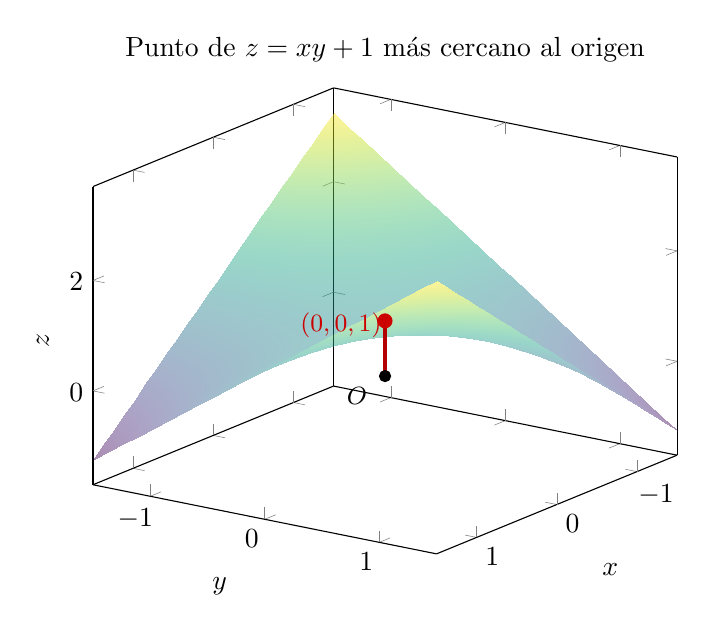
\begin{tikzpicture}
\begin{axis}[
    width=9cm, height=7.5cm,
    view={125}{22},
    colormap/viridis,
    xlabel={$x$}, ylabel={$y$}, zlabel={$z$},
    domain=-1.5:1.5, domain y=-1.5:1.5,
    samples=24, samples y=24,
    clip=false,
    title={Punto de $z=xy+1$ más cercano al origen},
]
    % Superficie z = xy + 1 (paraboloide hiperbólico desplazado)
    \addplot3[surf, opacity=0.45, shader=interp] {x*y + 1};
    % Origen
    \addplot3[only marks, mark=*, mark size=2pt, black]
        coordinates {(0,0,0)};
    \node at (axis cs:0.35,0,-0.15) [font=\small] {$O$};
    % Punto más cercano (0,0,1)
    \addplot3[only marks, mark=*, mark size=2.5pt, red!80!black]
        coordinates {(0,0,1)};
    \node at (axis cs:0.55,0,1.25) [font=\small, red!80!black] {$(0,0,1)$};
    % Segmento de distancia mínima
    \addplot3[red!70!black, ultra thick] coordinates {(0,0,0) (0,0,1)};
\end{axis}
\end{tikzpicture}
\end{center}

\subsection{Método para dos restricciones}

Cuando las variables deben satisfacer simultáneamente dos condiciones, $g(x, y, z) = k$ y $h(x, y, z) = m$, cada una define una superficie y su intersección es, en general, una curva $C$ en el espacio. El problema consiste en optimizar $f$ recorriendo esa curva.

\begin{mytheorem}{Multiplicadores de Lagrange (dos restricciones)}
Sean $f$, $g$ y $h$ con derivadas parciales continuas. Si $f$ alcanza un extremo local sobre la curva $C = \{g = k\} \cap \{h = m\}$ en un punto $P_0$ donde $\nabla g(P_0)$ y $\nabla h(P_0)$ son linealmente independientes, entonces existen escalares $\lambda$ y $\mu$ tales que:
\[
\nabla f(P_0) = \lambda\, \nabla g(P_0) + \mu\, \nabla h(P_0).
\]
\end{mytheorem}

Geométricamente, el vector tangente a la curva $C$ es perpendicular tanto a $\nabla g$ como a $\nabla h$. En un extremo, $\nabla f$ también debe ser perpendicular a esa tangente, y por lo tanto debe pertenecer al plano generado por $\nabla g$ y $\nabla h$. Esa condición de pertenencia se expresa como la combinación lineal $\nabla f = \lambda \nabla g + \mu \nabla h$.

El sistema resultante tiene cinco ecuaciones (tres de la condición vectorial y las dos restricciones) con cinco incógnitas: $x$, $y$, $z$, $\lambda$ y $\mu$.

\textbf{Ejemplo 3.} Encuentre los valores extremos de $f(x, y, z) = x + 2y + 3z$ sobre la curva intersección del plano $g(x, y, z) = x - y + z = 1$ y el cilindro $h(x, y, z) = x^2 + y^2 = 1$.

Los gradientes son:
\[
\nabla f = \langle 1, 2, 3 \rangle, \quad \nabla g = \langle 1, -1, 1 \rangle, \quad \nabla h = \langle 2x, 2y, 0 \rangle.
\]
La condición $\nabla f = \lambda \nabla g + \mu \nabla h$ da:
\[
1 = \lambda + 2\mu x, \qquad 2 = -\lambda + 2\mu y, \qquad 3 = \lambda.
\]
De la tercera, $\lambda = 3$. Sustituyendo en las dos primeras:
\[
1 = 3 + 2\mu x \;\Rightarrow\; \mu x = -1, \qquad 2 = -3 + 2\mu y \;\Rightarrow\; \mu y = \frac{5}{2}.
\]
Con $\mu \neq 0$: $x = -\dfrac{1}{\mu}$ y $y = \dfrac{5}{2\mu}$. La restricción del cilindro $x^2 + y^2 = 1$ da:
\[
\frac{1}{\mu^2} + \frac{25}{4\mu^2} = 1 \;\Rightarrow\; \frac{29}{4\mu^2} = 1 \;\Rightarrow\; \mu^2 = \frac{29}{4}, \quad \mu = \pm\frac{\sqrt{29}}{2}.
\]
Para $\mu = \dfrac{\sqrt{29}}{2}$: $x = -\dfrac{2}{\sqrt{29}}$, $y = \dfrac{5}{\sqrt{29}}$. El plano da $z = 1 - x + y = 1 + \dfrac{7}{\sqrt{29}}$. Entonces:
\[
f = x + 2y + 3z = -\frac{2}{\sqrt{29}} + \frac{10}{\sqrt{29}} + 3 + \frac{21}{\sqrt{29}} = 3 + \frac{29}{\sqrt{29}} = 3 + \sqrt{29}.
\]
Para $\mu = -\dfrac{\sqrt{29}}{2}$, un cálculo análogo da $f = 3 - \sqrt{29}$.

El máximo es $3 + \sqrt{29}$ y el mínimo es $3 - \sqrt{29}$, alcanzados en los dos puntos de la elipse intersección.

\begin{center}
\shorthandoff{>}
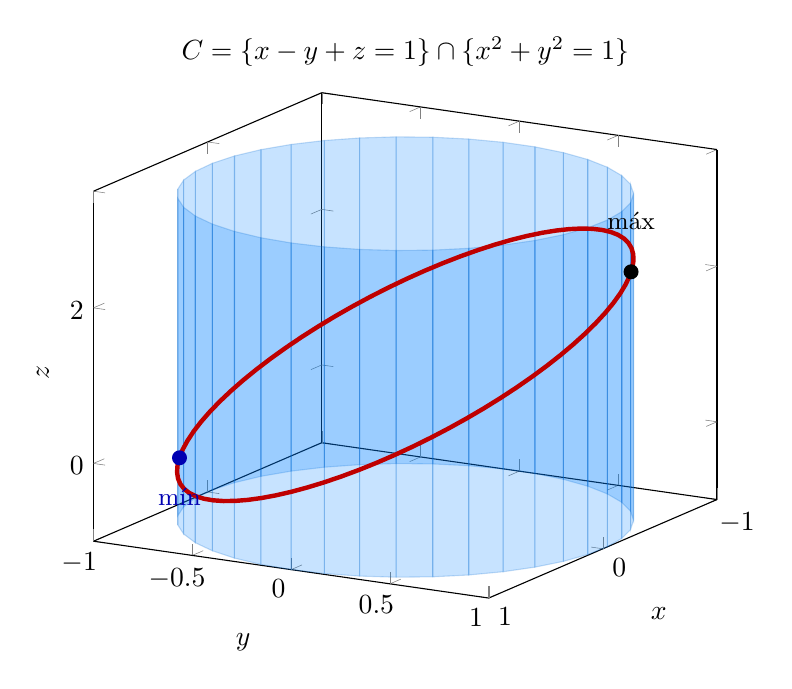
\begin{tikzpicture}
\begin{axis}[
    width=9.5cm, height=8cm,
    view={120}{18},
    xlabel={$x$}, ylabel={$y$}, zlabel={$z$},
    zmin=-1, zmax=3.5,
    clip=false,
    title={$C = \{x-y+z=1\} \cap \{x^2+y^2=1\}$},
]
    % Cilindro x^2+y^2=1 (paramétrico, semitransparente)
    \addplot3[surf, opacity=0.22, colormap/cool,
        domain=0:360, domain y=-1:3.2, samples=40, samples y=2,
        z buffer=sort]
        ({cos(x)}, {sin(x)}, {y});
    % Curva intersección: x=cos t, y=sin t, z=1-cos t+sin t
    \addplot3[red!75!black, ultra thick, domain=0:360, samples=80]
        ({cos(x)}, {sin(x)}, {1 - cos(x) + sin(x)});
    % Punto de máximo: x=-2/sqrt29≈-0.371, y=5/sqrt29≈0.928, z=1+7/sqrt29≈2.30
    \addplot3[only marks, mark=*, mark size=2.5pt, black]
        coordinates {(-0.371, 0.928, 2.300)};
    \node at (axis cs:-0.371,0.928,2.95) [font=\small] {máx};
    % Punto de mínimo: x=2/sqrt29≈0.371, y=-5/sqrt29≈-0.928, z=1-7/sqrt29≈-0.30
    \addplot3[only marks, mark=*, mark size=2.5pt, blue!70!black]
        coordinates {(0.371, -0.928, -0.300)};
    \node at (axis cs:0.371,-0.928,-0.80) [font=\small, blue!70!black] {mín};
\end{axis}
\end{tikzpicture}
\end{center}

La curva roja es la intersección del plano con el cilindro, una elipse en el espacio. Los puntos marcados son donde la función lineal $f$ alcanza sus valores extremos al recorrerla.

\subsection{Ejercicios}
\begin{enumerate}
    \item Use el método de los multiplicadores de Lagrange para encontrar los valores extremos de $f(x, y) = x^2 + y^2$ sujeto a la restricción $x^4 + y^4 = 1$.

    \item Encuentre los valores máximo y mínimo de $f(x, y) = 3x + 4y$ sobre la circunferencia $x^2 + y^2 = 1$. Interprete geométricamente el resultado en términos de la tangencia entre las rectas de nivel de $f$ y la circunferencia.

    \item Una caja rectangular sin tapa debe tener un volumen de $32\ \text{cm}^3$. Use multiplicadores de Lagrange para determinar las dimensiones que minimizan el área de material empleado.
\begin{enumerate}
    \item Plantee la función objetivo (área) y la restricción (volumen).
    \item Resuelva el sistema $\nabla A = \lambda \nabla V$ junto con la restricción.
    \item Determine las dimensiones óptimas y el área mínima.
\end{enumerate}

    \item Encuentre los puntos de la superficie $z^2 = xy + 4$ más cercanos al origen. Minimice el cuadrado de la distancia $f(x, y, z) = x^2 + y^2 + z^2$ sujeto a la restricción $g(x, y, z) = z^2 - xy = 4$.

    \item Encuentre los valores extremos de $f(x, y, z) = x + y + z$ sobre la curva intersección del cilindro $x^2 + y^2 = 2$ y el plano $y + z = 1$, usando el método de dos restricciones.

    \item Sean $a_1, a_2, \dots, a_n$ constantes positivas. Use multiplicadores de Lagrange para demostrar que el máximo de $f(x_1, \dots, x_n) = \sum_{i=1}^{n} a_i x_i$ sujeto a $\sum_{i=1}^{n} x_i^2 = 1$ es $\sqrt{\sum_{i=1}^{n} a_i^2}$, y que se alcanza cuando $\mathbf{x}$ es paralelo al vector $\langle a_1, \dots, a_n \rangle$. Este resultado equivale a la desigualdad de Cauchy-Schwarz.

\end{enumerate}